% Ubah judul dan label berikut sesuai dengan yang diinginkan.
\section{Hasil dan Pembahasan}
\label{sec:hasildanpembahasan}

\subsection{Visualisasi Hasil Kalibrasi}
\label{sec:visualisasihasil} 

Visualisasi hasil kalibrasi dilakukan dengan cara data pada kamera dengan data pada lapangan. Hal itu dilakukan dengan cara memasukkan data pada kamera ke dalam \emph{Lookup Table} yang telah dibuat sebelumnya. Berikut adalah hasil visualisasi yang didapat. 

\begin{figure}[ht]
  \centering
  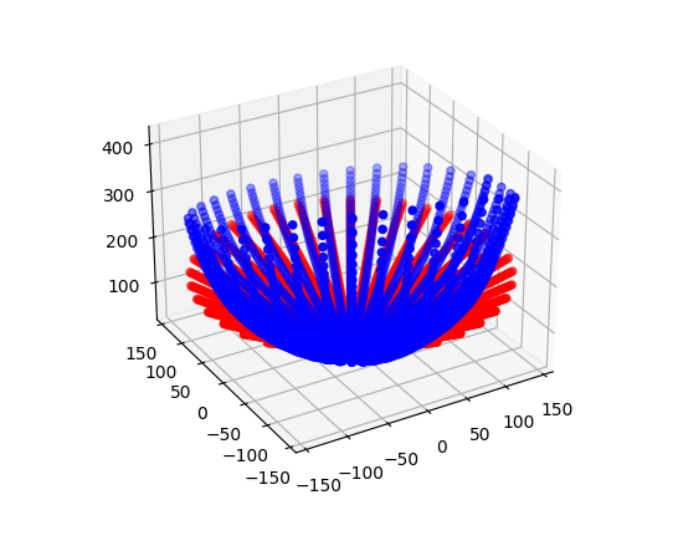
\includegraphics[width=8cm]{gambar/visual1.png}
  \caption{Visualisasi hasil kalibrasi.}
  \label{fig:hasilkalibrasi}
\end{figure}

Dari gambar tersebut, dapat dilihat bahwa data pada kamera yang digunakan tidak sepenuhnya diproyeksikan tegak lurus 90 derajat dengan lapangan. Hal itu terjadi karena kamera yang digunakan tidak terpasang dengan benar. 

\subsection{Skenario Pengujian Akurasi}
\label{sec:skenariopengujian}

Pengujian dilakukan dengan cara mendeteksi bola yang diam di lapangan dengan memutar robot pada posisinya sendiri. Hal itu membuat robot dapat melihat bola dari berbagai sudut. Pengujian dilakukan dengan mengambil data dari kamera omnivision yang telah terpasang pada robot lalu memroses data tersebut menggunakan \emph{Lookup Table} yang telah dibuat sebelumnya sehingga didapat koordinat bola pada lapangan. Berikut adalah skenario pengujian yang dilakukan: 

\begin{figure}[ht]
  \centering
  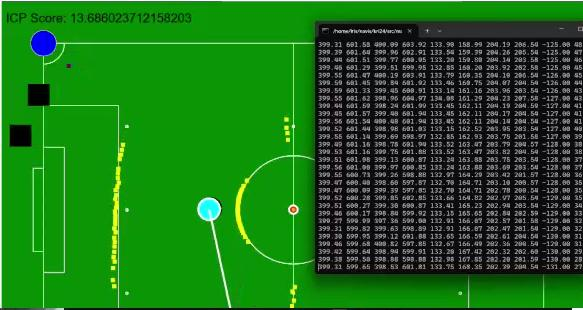
\includegraphics[width=8cm]{gambar/saat_putar_bola_2.jpeg}
  \caption{Skenario Pengujian.}
  \label{fig:skenariopengujian}
\end{figure}

Prosedur tersebut dilakukan pada jarak robot dengan bola pada lapangan yang berbeda-beda yaitu pada 120 cm, 200 cm, dan 285 cm. 

Adapun rumusan yang digunakan untuk menghitung posisi bola pada lapangan adalah sebagai berikut: 

\begin{equation}
  \begin{aligned}
    dx &= x\_bola\_cam - x\_center\_cam \\
    dy &= y\_center\_cam - y\_bola\_cam \\
    r\_bola\_cam &= \sqrt{dx^2 + dy^2} \\
    \theta\_bola\_cam &= \arctan(\frac{dy}{dx}) \\
    index &= \theta\_bola\_cam \times r\_max + r\_bola\_cam \\ 
    r\_bola\_lap &= r\_lookup[index] \\
    \theta\_bola\_lap &= \theta\_bola\_cam + robot\_pose\_\theta - 90 \\
    x\_bola &= robot\_pose\_x + r\_bola\_lap \times \cos(\theta\_bola\_lap) \\
    y\_bola &= robot\_pose\_y + r\_bola\_lap \times \sin(\theta\_bola\_lap) \\
  \end{aligned}
\end{equation}

\subsection{Evaluasi Pengujian Akurasi}
\label{sec:analisispengujian}

Dari pengujian yang telah dilakukan, didapat data sebagai berikut:

% Contoh pembuatan tabel
\begin{table}[htbp]
  \caption{Hasil Pengujian Posisi Bola pada Lapangan dengan Jarak 120 cm.}
  \begin{center}
    \begin{tabular}{|c|c|c|}
      \hline
    \rowcolor[HTML]{C0C0C0}
  \textbf{Sudut Robot ke Bola} & \textbf{Posisi Bola X} & \textbf{Posisi Bola Y} \\
  \hline

  0 deg            & 407.74 cm                & 596.67 cm            \\
  30 deg           & 409.41 cm                & 600.3 cm            \\
  60 deg           & 409.65 cm                & 600.54 cm            \\
  90 deg           & 407.52 cm                & 598.2 cm           \\
  120 deg           & 407.18 cm                & 600.07 cm           \\
  150 deg           & 409.98 cm                & 598.35 cm           \\
  180 deg           & 410.66 cm                & 593.41 cm           \\
  210 deg           & 410.84 cm                & 590.28 cm           \\
  240 deg           & 410.01 cm                & 590.8 cm           \\
  270 deg           & 409.9 cm                & 594.28 cm           \\
  300 deg           & 408.91 cm                & 590.14 cm           \\
  330 deg           & 408.8 cm                & 591.57 cm           \\
  \hline
\end{tabular}
\end{center}
\end{table}

\begin{table}[htbp]
  \caption{Hasil Pengujian Posisi Bola pada Lapangan dengan Jarak 200 cm.}
  \begin{center}

  \begin{tabular}{|c|c|c|}
  \hline
  \rowcolor[HTML]{C0C0C0}
  \textbf{Sudut Robot ke Bola} & \textbf{Posisi Bola X} & \textbf{Posisi Bola Y} \\
  \hline
  0 deg            & 406.44 cm                & 613.13 cm            \\
  30 deg           & 411.09 cm                & 624.66 cm            \\
  60 deg           & 416.39 cm                & 627.02 cm            \\
  90 deg           & 411.55 cm                & 625.85 cm           \\
  120 deg           & 408.85 cm                & 620.01 cm           \\
  150 deg           & 414.2 cm                & 611.7 cm           \\
  180 deg           & 415.12 cm                & 601.25 cm           \\
  210 deg           & 412.78 cm                & 592.09 cm           \\
  240 deg           & 410.77 cm                & 594.57 cm           \\
  270 deg           & 409.66 cm                & 598.43 cm           \\
  300 deg           & 407.92 cm                & 599.03 cm           \\
  330 deg           & 406.29 cm                & 602.72 cm           \\
  \hline
\end{tabular}
\end{center}
\end{table}

\begin{table}[htbp]
\caption{Hasil Pengujian Posisi Bola pada Lapangan dengan Jarak 285 cm.}
\begin{center}
  
\begin{tabular}{|c|c|c|}
  \hline
  \rowcolor[HTML]{C0C0C0}
  \textbf{Sudut Robot ke Bola} & \textbf{Posisi Bola X} & \textbf{Posisi Bola Y} \\
  \hline
  0 deg            & 380.98 cm                & 593.81 cm            \\
  30 deg           & 382.14 cm                & 594.49 cm            \\
  60 deg           & 383.41 cm                & 607.18 cm            \\
  90 deg           & 392.49 cm                & 604.67 cm           \\
  120 deg           & 390.32 cm                & 606.04 cm           \\
  150 deg           & 391.43 cm                & 598.47 cm           \\
  180 deg           & 387.17 cm                & 587.89 cm           \\
  210 deg           & 390.16 cm                & 577.15 cm           \\
  240 deg           & 389.67 cm                & 585.82 cm           \\
  270 deg           & 389.38 cm                & 590.31 cm           \\
  300 deg           & 382.61 cm                & 593.25 cm           \\
  330 deg           & 380.73 cm                & 589.31 cm           \\
  \hline
\end{tabular}
\end{center}
\end{table}


Dari tabel tersebut didapat standar deviasi pada data posisi bola pada lapangan dengan jarak 120 cm adalah 1.26 cm dan 4.11 cm untuk posisi bola x dan y. Sedangkan pada jarak 200 cm didapat standar deviasi 3.28 cm dan 12.80 cm untuk posisi bola x dan y. Pada jarak 285 cm didapat standar deviasi 4.40 cm dan 8.92 cm untuk posisi bola x dan y. 

Dari hasil tersebut dapat disimpulkan bahwa sistem kalibrasi yang telah dibuat dapat mendeteksi posisi bola pada lapangan dengan baik. Bola tidak tepat berada di tengah lapangan bisa disebabkan oleh beberapa faktor. Adapun beberapa faktor penyebabnya adalah ketidaktepatan posisi bola pada dunia aslinya, ketidaktepatan posisi robot pada dunia aslinya, dan ketidaktepatan orientasi robot pada dunia aslinya. Karena pada dasarnya sesuai dengan rumus \textbf{4.1}, posisi bola pada lapangan juga ditentukan oleh posisi robot pada lapangan. 

\subsection{Skenario Pengujian Akurasi Kedua}
\label{sec:skenariopengujian2}

Pengujian akurasi kedua adalah dengan cara membandingkan hasil kalibrasi baru dengan kalibrasi lama yang masih menggunakan algoritma \emph{regresi polynomial}. Pengujian dilakukan dengan cara yang sama seperti pengujian akurasi sebelumnya. Namun, proses perhitungannya menggunakan algoritma \emph{regresi polynomial}. 

\subsection{Evaluasi Pengujian Akurasi Kedua}
\label{sec:analisispengujian2}
\begin{table}[htbp]

\caption{Hasil Pengujian Posisi Bola pada Lapangan dengan Jarak 120 cm menggunakan Kalibrasi Lama.}
\begin{center}
  

\begin{tabular}{|c|c|c|}
  \hline
  \rowcolor[HTML]{C0C0C0}
  \textbf{Sudut Robot ke Bola} & \textbf{Posisi Bola X} & \textbf{Posisi Bola Y} \\
  \hline
  0 deg            & 370.18 cm                & 576.31 cm            \\
  30 deg           & 376.24 cm                & 585.42 cm            \\
  60 deg           & 383.91 cm                & 597.98 cm            \\
  90 deg           & 392.99 cm                & 605.67 cm           \\
  120 deg           & 390.23 cm                & 610.94 cm           \\
  150 deg           & 400.49 cm                & 598.89 cm           \\
  180 deg           & 385.97 cm                & 582.89 cm           \\
  210 deg           & 398.61 cm                & 577.15 cm           \\
  240 deg           & 390.76 cm                & 585.02 cm           \\
  270 deg           & 386.32 cm                & 588.91 cm           \\
  300 deg           & 378.69 cm                & 585.55 cm           \\
  330 deg           & 370.32 cm                & 579.11 cm           \\
  \hline
\end{tabular}
\end{center}
\end{table}

Dari data tersebut dapat dilihat bahwa standar deviasi pada data posisi bola pada lapangan dengan jarak 120 cm menggunakan kalibrasi lama adalah 10.01 cm dan 11.32 cm untuk posisi bola x dan y. Sedangkan pada kalibrasi baru standar deviasi 1.26 cm dan 4.11 cm untuk posisi bola x dan y. Dapat dilihat bahwa kalibrasi baru lebih baik dibandingkan dengan kalibrasi lama. Hal itu terjadi karena pemasangan kamera pada robot yang tidak tepat sehingga menyebabkan hasil kalibrasi lama menjadi tidak akurat. Ketidakakuratan tersebut terjadi karena kalibrasi lama hanya menggunakan satu arah saja sebagai referensi untuk model regresi polynomial. Sedangkan, pada kenyataannya rumus model untuk masing-masing arah kamera akan selalu berbeda.  

\subsection{Skenario Pengujian Kecepatan Komputasi}
\label{sec:analisispengujian}

Pengujian dilakukan dengan cara membandingkan apakah sistem kalibrasi baru lebih cepat dibandingkan menggunakan sistem kalibrasi lama. Pengujian dilakukan dengan cara mencatat waktu setelah kalibrasi lalu menguranginya dengan waktu sebelum kalibrasi. Sehingga bisa didapat perkiraan waktu lamanya sistem melakukan proses perhitungan untuk melakukan kalibrasi. Berikut rumus yang digunakan untuk menghitung waktu delay: 

\begin{equation}
  \begin{aligned}
    delay\_time &= waktu1 - waktu0 \\ 
  \end{aligned}
\end{equation}

Dimana $waktu1$ adalah waktu setelah kalibrasi dan $waktu0$ adalah waktu sebelum kalibrasi.


\subsection{Evaluasi Pengujian Kecepatan Komputasi}
\label{sec:analisispengujian}

Dari pengujian yang telah dilakukan, didapat data sebagai berikut: 

\begin{table}{|c|c|c|}
  \caption{Hasil Pengujian Perbedaan Kecepatan Komputasi}
\begin{center}
  

\begin{tabular}{|c|c|c|}
  \hline
  \rowcolor[HTML]{C0C0C0}
  \textbf{Iterasi ke-} & \textbf{Waktu Kalibrasi Baru} & \textbf{Waktu Kalibrasi lama} \\
  \hline
  0            & 119 ns                & 176 ns            \\
  1           & 76 ns                & 86 ns            \\
  2           & 25 ns                & 107 ns            \\
  3           & 31 ns                & 90 ns           \\
  4           & 32 ns                & 88 ns           \\
  5           & 36 ns                & 87 ns           \\
  6           & 37 ns                & 88 ns           \\
  7           & 34 ns                & 93 ns           \\
  8           & 37 ns                & 89 ns           \\
  9           & 35 ns                & 90 ns           \\
  \hline
\end{tabular}
\end{center}
\end{table}

Dari grafik tersebut dapat dilihat bahwa sistem kalibrasi baru lebih cepat 53.2 ns dibandingkan dengan sistem kalibrasi lama. Dengan rata-rata Kalibrasi baru membutuhkan waktu 46.2 ns sedangkan kalibrasi lama membutuhkan waktu 99.4 ns. Hal tersebut disebabkan karena sistem kalibrasi baru hanya menggunakan \emph{Lookup Table} yang berisi data kalibrasi kamera. Sedangkan sistem kalibrasi lama menggunakan algoritma \emph{regresi polynomial} yang membutuhkan waktu lebih lama.